\chapter{Theoretical background}
\label{cha:theoreticalBackground}

\section{Semantic Web}
\label{sec:semanticWeb}

\subsection{Background}
\label{sub:semWebBackground}

Today's World Wide Web has achieved a great success. WWW is widely used all around the world. Simple foundations, on which it is based, has given its strength and global community. Almost every user is able to create and publish hypertext resources in a simple manner. Basically \textit{"web content consists mainly of distributed hypertext, and is accessed via a combination of keyword-based search and link navigation"} \cite{HorSSF}.

Notably, upon explosion of information amount accessible through the web, current web has encountered drawbacks. The huge amount of content required to be processed in order to find desired facts, has \textit{"highlighted some serious shortcomings in the hypertext paradigm"} \cite{HorSSF}:
\begin{itemize}
    \setlength{\itemsep}{0cm}
    \setlength{\parskip}{0cm}

    \item difficulties in finding correct information through simple searching and browsing mechanisms,
    \item problems of finding facts, which has common correspondents,
    \item irrelevant results after providing of more complex queries in the browsing engines,
    \item lack of semantics,
    \item lack of deduction facilities.
\end{itemize}

\noindent People are facing inconveniences in web content browsing. It is obvious, that content processing tasks are much more complicated when it comes to implement them into software agents. It is because technologies used for hypertext documents creation are designed with the intention of describing and presenting information in the human way. The lack of formal, logic-based information structure is the big issue for machines, which require mathematically-based way for knowledge processing. Here are the challenges, current web is going to face.

\newpage

\subsection{Evolution}
\label{sub:semWebEvolution}

Today's World Wide Web gives new opportunities for discipline called Knowledge Representation (KR). Web resources needs to be better adopted for automatic processing by computer agents. That is possible by more systematic and formal description mechanisms used for defining contents of the pages. What is more, Uniform Resource Identifiers (URIs), which are the naming scheme for web resources, allows KR systems to improve linking between semantic documents by avoiding the ambiguities of natural language. That is why new possibilities and challenges are opened for knowledge representation assumptions \cite{HLP08}.

One of the most powerful feature of the World Wide Web is the possibility of interconnections between knowledge sources. Interconnections are provided by linking mechanisms on pages. In other words, instead of copying information from external sources created by other people to our page, we just provide links to such sources.

Semantic Web can be treated as an extension to current web and the successor of Web 2.0. In recent Web 2.0 architecture, there is a lot of unstructured data. Information is represented in various ways, incompatible witch each other. What Semantic Web offers is defined meaning of information, machine-readable description of contents, simplification of information exchange, classification and inference mechanisms, data processing and integration in machine-automated manner. 

\medskip

\begin{figure}[htp]
\centering
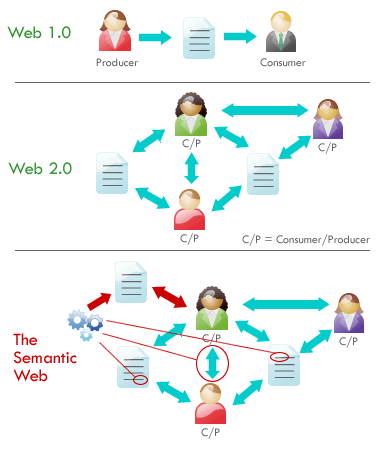
\includegraphics[scale=0.65]{images/chapter2/WebEvolution}
\caption{Web evolution from old Web 1.0 up to Semantic Web \cite{PWGB}}
\label{fig:webEvolution}
\end{figure}

\newpage

\subsection{Outline}
\label{sub:semWebOutline}

\noindent \textit{"The Semantic Web is an extension of the current Web in which information is given well-defined meaning, better enabling computers and people to work in cooperation."} 
\begin{flushright} Tim Berners-Lee \cite{BHL01} \end{flushright}

\noindent \textit{"The goal of Semantic Web research is to transform the Web from a linked document repository into a distributed knowledge base and application platform, thus allowing the vast range of available information and services to be more effectively exploited."} 
\begin{flushright} Ian Horrocks \cite{HorSSF} \end{flushright}

\noindent The Semantic Web is not about links between web pages, but about relationships between things (e.g. A is a part of B and Y is a member of Z) and about properties of things (e.g. size, weight, age and price) \cite{SemWebTutorial}.

\bigskip

\noindent \textit{"If HTML and the Web made all the online documents look like one huge book, RDF, schema, and inference languages will make all the data in the world look like one huge database."}
\begin{flushright} Tim Berners-Lee \cite{BLF99} \end{flushright}

\noindent As it was said, the Semantic Web is a web that is able to provide information about things in the way computers can understand. The human-understandable sentences which describe things, are going to be intelligently processed in the Semantic Web. 

Statements appropriate for dedicated language are built using syntax rules, which are defined by this language. In Semantic Web field statements are built using rules provided by specific KR languages and such statements are semantic aware. Semantic analysis of such statements allows to convert them to knowledge base queries. To search and access the Semantic Web content, tools called \textit{Semantic Web Agents} or \textit{Semantic Web Services} are required. It is because searching process in Semantic Web will be much different than today's searching in free text - complicated math algorithms are going to find answers for us.

\bigskip

\noindent \textit{"The Semantic Web provides a common framework that allows data to be shared and reused across application, enterprise, and community boundaries."}
\begin{flushright} World Wide Web Consortium \cite{SemWebActivity} \end{flushright}

\newpage

\noindent The Semantic Web layered architecture (Figure \ref{fig:semWebStack}) covers such technological aspects like application interfaces, security, rules and logic (SWRL, RIF), ontologies (RDFS, OWL), metadata (RDF), serialization (XML) and resource identification (URI).

\medskip

\begin{figure}[htp]
\centering
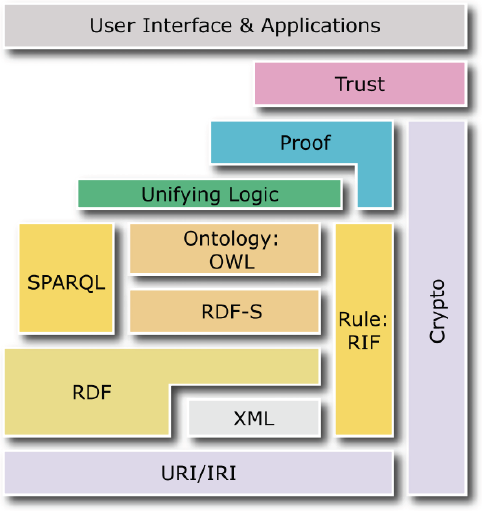
\includegraphics[scale=0.6]{images/chapter2/SemanticWebStack}
\caption{Semantic Web Stack \cite{GJNSemWeb}}
\label{fig:semWebStack}
\end{figure}

\subsubsection{KR languages and tools}
\label{sss:krLanguagesAndTools}

The KR languages: RDF, RDFS and OWL explained in the next sections, are \textit{"without question the most widely used KR languages in history"} \cite{HLP08}. They were created to capture and describe knowledge gathered by the web resources, and help applications to use these resources in an intelligent way. These languages are shaping the new standards in web development, allowing for transformation to the new standards. The Web 3.0 is slowly coming to light.

Along with the mentioned languages, development of new tools cooperating with them has appeared. Tools are designed for creating and maintaining taxonomies, and are supported by DL reasoning services (see Section \ref{sub:owlAndReasoners}). It gives the wide group of Semantic Web community new possibilities and motivation for creation ontology-based applications and experimenting with that technology. New challenges have appeared such as large scale OWL-based applications development.

\newpage

\section{Towards ontology development}
\label{sec:towardsOntologyDevelopment}

\subsection{Introduction}
\label{sub:towardsOntologiesDevelopmentIntroduction}

\textit{"In recent years the development of ontologies has been moving from the realm of Artificial-Intelligence laboratories to the desktops of domain experts"} \cite{OntDev101}. Many organizations and disciplines has developed standardized ontologies that domain experts can exchange and reuse in building their own ones. An ontology, \textit{"explicit formal specifications of the terms in the domain and relations among them"} \cite{Gru93}, specifies set of common vocabulary, researchers can share within a domain of knowledge. Ontologies have become increasingly important with the global move towards the Semantic Web. Parallel with Semantic Web evolution, knowledge defined by ontologies can be available on the web to a multitude of machines. 

\subsection{Reasons and advantages}
\label{sub:reasonsAndAdvantages}

The key reasons for developing an ontology \cite{OntDev101} are following:
\begin{enumerate}
    \setlength{\itemsep}{0cm}
    \setlength{\parskip}{0cm}

    \item To share common understanding of the structure of information among people or software agents.
    \item To enable reuse of domain knowledge.
    \item To make domain assumptions explicit.
    \item To separate domain knowledge from the operational knowledge.
    \item To analyze domain knowledge.
\end{enumerate}

Ad 1. Sharing common understanding of knowledge domain is one of the most critical reason for developing ontologies. For example, we can imagine several web sites containing specific technical information. If that information is published under common comprehensive ontology, the software agents will be able to aggregate and process knowledge from them, and infer exhaustive answers for user queries to that domain. 

Ad 2. Coherent domain knowledge sharing, along with reusing of such knowledge can provide the possibility of injecting new aspects in existing set of information. This possibility, will provide complex description of specific knowledge structures to researchers all around the world, where one team of experts can supplement existing structure with new elements, with standardized vocabulary set. Along with automatic processing of knowledge, answering to questions about domain related topics, is going to be coherent and comprehensive.

Ad 3. Explicit domain assumptions provide clear description of domain knowledge, and simplify knowledge extensibility for domain. New researchers have the possibility of view to comprehensive domain related information structure, and while learning about that structure, have easier task in understanding what specific terms mean. Besides, in the world of software applications, explicit assumptions are much better than hard coded assumptions. Hard coded information along with all relations, would be much harder to find, and any changes would be impossible to execute, without programming expertise.

Ad 4. When it comes to separation, between domain knowledge and operational knowledge, we can talk about some kind of loose coupling between them. We can develop abstract set of assumptions in the domain, and next use that metadata for providing specific, context-based information about such domain. For example domain experts can research an ontology which describe traffic dangers aspect, and users can provide specific traffic danger information for that underlying ontology, by defining concrete locations where specific traffic conditions can appear.

Ad 5. Analyzing domain knowledge is an obvious value on its own. It is critical when it comes to extend existing, or providing new branches of specific domain. Analysis should be based on comprehensive, structured source of knowledge, which an ontology is, and should provide an easy way of global view of concept along with description of all related terms used to define it.

\bigskip

\noindent Similar classification provided by The Knowledge Systems, AI Laboratory (KSL) at Stanford University \cite{KSL} is following:
\begin{itemize}
    \setlength{\itemsep}{0cm}
    \setlength{\parskip}{0cm}

    \item to enable a machine to use the knowledge in some application,
    \item to enable multiple machines to share their knowledge,
    \item to help yourself understand some area of knowledge better,
    \item to help other people understand some area of knowledge,
    \item to help people reach a consensus in their understanding of some area of knowledge.
\end{itemize}

\noindent These particular points, in a bit different form, were described earlier. Ontology development aims, described by different sources, are convergent. Ontologies development seems to be crucial in the near future, because the size of human knowledge is going to be too wide for processing in the meaning of standard way.

\newpage

\section{XML}
\label{sec:xml}

\subsection{Introduction}
\label{sub:xmlIntroduction}

The starting point of introduction to world of KR languages, should be brief description of XML language. It is because XML lies on the bottom of Semantic Web layered stack and provides the serialization for mentioned KR languages.

XML is widely used technology so information stored in variety of papers, e.g. \cite{W3SchoolsXML, W3CXML}, can be easily found to help understand, what exactly is XML.

\bigskip

\noindent XML facts:
\begin{itemize}
    \setlength{\itemsep}{0cm}
    \setlength{\parskip}{0cm}

    \item XML stands for EXtensible Markup Language,
    \item XML is a markup language much like HTML,
    \item XML allows to represent tree-like structures,
    \item XML was designed to carry data, not to display data,
    \item XML tags are not predefined - custom tags have to be defined,
    \item XML is designed to be self-descriptive,
    \item XML is platform independent,
    \item XML files are stored as plain text files,
    \item XML emphasizes simplicity, generality, and usability over internet,
    \item XML is a W3C Recommendation.
\end{itemize}

\noindent XML is used in many various aspects of coherent data transmission through the web. In the real world incompatible data formats coexist in computer systems, and are completely incomprehensible to each other. XML provides common, interchangeable way of storing and sharing data. It is a software and hardware independent tool for carrying information. It is also used as the serialization mechanism for various, newly created internet languages like: XHTML, WSDL (describing Web Services), RSS (used for news feeds), RDF and OWL (describing resources and ontologies), SMIL (describing multimedia for the web), etc.

\newpage

\noindent Below, there is a sample XML document:

{\tt \small
\begin{verbatim}
<?xml version="1.0" encoding="UTF-8"?>
<message status="critical" releaseDate="13th April, 1970">
   <to>Manned Spacecraft Center (building 30), Houston, Texas</to>
   <from>Commander James A. Lovell, Apollo 13 crew</from>
   <heading>Technical Fault</heading>
   <body>
      Houston, we've had a problem. 
      We've had a main B bus undervolt.
   </body>
</message>
\end{verbatim}
}

\noindent First line of the file indicates, that it is version 1.0 of XML standard, and information is encoded with UTF-8 character encoding. File content declares a message sent on the 13th of April, 1970, from Apollo 13 spacecraft to mission control center, about technical issue connected with oxygen tank explosion. 

This document is quite self-descriptive. It contains sender and receiver information, heading and the message body. Notably, that piece of code does not provide any functionality, besides carrying and structuralizing the data. It is just information wrapped in tags. There is still a necessity for writing software which will be able to process and respond, or display that information in more friendly way.

\subsection{XML syntax}
\label{sub:xmlSyntax}

\subsubsection{Elements}
\label{sss:xmlElements}

The tags used inside XML documents, are not defined in any XML standard. XML allows developers to invent custom tags, because as opposed to HTML where tags are the part of the standard, XML has no predefined tags.

XML documents have to contain one root element. Structure of XML documents is the structure of rooted tree. The tree starts at the root and branches to the lowest level of the tree. A rooted tree is a connected, acyclic, undirected graph, in which one of the vertices is distinguished from others. The distinguished vertex is called the root of the tree \cite{CLR90}.

\newpage

{\tt \small
\begin{verbatim}
<root>
   <firstChild>
      <subChild>.....</subChild>
   </firstChild>
   <secondChild>
      <subChild>.....</subChild>
   </secondChild>
</root>
\end{verbatim}
}

\noindent An XML element is everything from (including) the element start tag to (including) the element end tag. Elements can contain other elements, plain text or a mixture of both. Each XML tag have to close previously opened tag, in the correct order. It is illegal to have unclosed tag in XML document. All elements must be properly nested. What is more, XML is case sensitive.

{\tt \small
\begin{verbatim}
<p>incorrect - no closing tag
<p>correct</p>

<p><b>incorrect - improperly nested elements</p></b>
<p><b>correct</b></p>

<P>incorrect - tags are not matched in the manner of case sensitivity</p>
<P>correct</P>
<p>correct</p>
\end{verbatim}
}

\subsubsection{Attributes}
\label{sss:xmlAttributes}

XML elements can have attributes. Attributes provide additional information about elements. Attribute is a simple key-value pair, in the format of \textit{key="value"}. Attribute values have to be quoted.

{\tt \small
\begin{verbatim}
<message status="critical">.....</message>
\end{verbatim}
}

\noindent There are some problems with attributes. In opposite to elements they cannot contain multiple values, as well as tree structures. They are not easily expandable for future changes. 

\setlist{nosep} % eliminate space before \begin{itemize}
\begin{framed}
\begin{itemize}
    \setlength{\itemsep}{0cm}
    \setlength{\parskip}{0cm}

    \item Attributes should be used for providing information, which is not relevant to the data itself. They are excellent for storing \textit{metadata} (data about data) (such as ID of message, etc.).
    \item For storing \textit{data itself}, elements are much better choice than attributes.
\end{itemize}
\end{framed}
\setlist{} % revert nosep for subsequent lists

\newpage

\subsubsection{Others}
\label{sss:xmlOthers}

XML supports comments. The syntax for writing comments in XML is similar to that of HTML:

{\tt \small
\begin{verbatim}
<!-- This is a comment --> 
\end{verbatim}
}

\noindent Some characters in XML Standard have special purpose. It means, that XML parsers try to interpret such characters in a special way. To insert such a character in the XML document without its meaning, predefined entity references should be used:

\medskip

\begin{table}[htp]
\centering
\begin{tabular}{ |>{\tt}p{2cm}|>{\tt}l|l| }
    \hline
    \&lt;       & <     & less than \\ \hline
    \&gt;       & >     & greater than \\ \hline
    \&amp;      & \&    & ampersand \\ \hline
    \&apos;     & '     & apostrophe \\ \hline
    \&quot;     & "     & quotation mark \\ \hline
\end{tabular}
\caption{Predefined entities in XML 1.0}
\end{table}

\noindent As opposed to HTML, white-space characters in XML document are NOT truncated. When it comes to storing new lines, XML behaves in the same way as Unix/Mac applications, and uses line feed character (LF).

XML documents can follow a set of strict rules, to store information in a predefined format. If they follow such rules, they are \textit{valid}. Such predefined data structure is critical during parsing of XML documents by various applications. It helps applications to properly interpret specific information, because when transporting data, it is essential that both sender and receiver have the same "expectations" about the content. If XML document doesn't follow its schema, it can be rejected by application as invalid. 

\subsection{Structure and content validation}
\label{sub:dtd}

The standard defining syntax rules which should be followed by XML documents is called Document Type Definition (DTD). It describes the structure with a list of legal tags and their attributes. DTD can be embedded within XML file: 

\newpage

{\tt \small
\begin{verbatim}
<?xml version="1.0" encoding="UTF-8"?>
<!DOCTYPE message [
<!ELEMENT message (to,from,heading,body)>
<!ATTLIST message status (spam|normal|critical) "spam">
<!ATTLIST message releaseDate CDATA #REQUIRED>
<!ELEMENT to (#PCDATA)>
<!ELEMENT from (#PCDATA)>
<!ELEMENT heading (#PCDATA)>
<!ELEMENT body (#PCDATA)>
]>
<message status="critical" releaseDate="13th April, 1970">
   <to>Manned Spacecraft Center (building 30), Houston, Texas</to>
   <from>Commander James A. Lovell, Apollo 13 crew</from>
   <heading>Technical Fault</heading>
   <body>
      Houston, we've had a problem. 
      We've had a main B bus undervolt.
   </body>
</message>
\end{verbatim}
}

\noindent or can exist as a separate file, which can be referenced from the XML document, as marked out below:

{\tt \small
\newcommand\codeHighlight[1]{\textcolor[rgb]{1,0,0}{\textbf{#1}}}
\begin{Verbatim}[commandchars=\\\{\}]
<?xml version="1.0" encoding="UTF-8"?>
\textbf{<!DOCTYPE message SYSTEM "\codeHighlight{message.dtd}">}
<message status="critical" releaseDate="13th April, 1970">
   <to>Manned Spacecraft Center (building 30), Houston, Texas</to>
   <from>Commander James A. Lovell, Apollo 13 crew</from>
   <heading>Technical Fault</heading>
   <body>
      Houston, we've had a problem. 
      We've had a main B bus undervolt.
   </body>
</message>
\end{Verbatim}
}

\noindent More powerful XML-based alternative to DTD is called XML Schema. The migration from older DTDs to XML Schema includes following benefits:
\begin{itemize}
    \setlength{\itemsep}{0cm}
    \setlength{\parskip}{0cm}

    \item Schemas support primitive (built-in) data types (e.g. \texttt{xsd:integer}, \texttt{xsd:string}, \texttt{xsd:date}, etc.) and data namespaces.
    \item Schemas are extensible. Schemas gives possibility of defining custom data types, using object-oriented data modeling principles: encapsulation, inheritance and substitution.
    \item It is possible to reuse them in other Schemas, create new data types derived from the standard types and reference multiple schemas within the same document.
    \item Schemas are compatible with other XML technologies (Web Services, XQuery, XSLT, etc.).
\end{itemize}

\noindent Sample schema shown below, can be used as an alternative to DTD introduced earlier, for defining the syntactic correctness of XML document also discussed earlier:

{\tt \small
\begin{verbatim}
<xs:element name="message">
   <xs:complexType>
      <xs:sequence>
         <xs:element name="to" type="xs:string"/>
         <xs:element name="from" type="xs:string"/>
         <xs:element name="heading" type="xs:string"/>
         <xs:element name="body" type="xs:string"/>
      </xs:sequence>
      <xs:attribute name="status" type="xs:string" default="spam"/>
      <xs:attribute name="releaseDate" type="xs:string" use="required"/>
   </xs:complexType>
</xs:element>
\end{verbatim}
}

\section{RDF}
\label{sec:rdf}

\subsection{Introduction}
\label{sub:rdfIntroduction}

If we take a look once again at Semantic Web Stack, we can see that just above XML lies Resource Description Framework (RDF). RDF is a simple assertional language used for describing resources in the World Wide Web. RDF is intended for situations where information is processed in automatic manner by applications, rather than being displayed to users. It is designed to represent information in the form of \textbf{triples}, such as \textit{subject}, \textit{predicate} and \textit{object}. RDF predicates can be treated as attributes of resources. Sample \textbf{subject-predicate-object} (object-attribute-value) triple building block is shown on the directed graph below:

\medskip

\begin{figure}[htp]
\centering
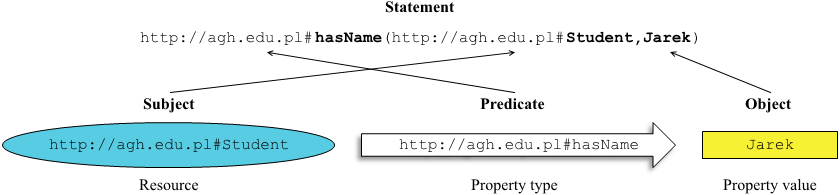
\includegraphics[scale=0.72]{images/chapter2/RDFTriple}
\caption{Example of RDF statement}
\label{fig:rdfTriple}
\end{figure}

\newpage

\noindent Resources refers to things being described. Resources are identified by URIs. The binary relations between resources are called properties. RDF properties themselves also have URIs, to be more accurate in the identification of the relations between resources. Statements are created as the asserted properties of resources.

\subsection{RDF syntax}
\label{sub:rdfSyntax}

RDF provides XML-based syntax, called RDF\slash XML. A piece of RDF\slash XML code written below corresponds to the graph in Figure \ref{fig:rdfTriple}:

{\tt \small
\begin{verbatim}
1. <?xml version="1.0"?>
2. <rdf:RDF xmlns:rdf="http://www.w3.org/1999/02/22-rdf-syntax-ns#"
3.          xmlns:agh="http://agh.edu.pl#">

4.    <rdf:Description rdf:about="http://agh.edu.pl#Student">
5.       <agh:hasName>"Jarek"</agh:hasName>
6.    </rdf:Description>

7. </rdf:RDF>
\end{verbatim}
}

\noindent Line numbers are added to the example. It is because they are referenced in the explanation part below:
\begin{itemize}
    \setlength{\itemsep}{0cm}
    \setlength{\parskip}{0cm}

    \item \textit{Line 1} contains standard XML declaration \texttt{<?xml version="1.0"?>}, which indicates that the content of that file is XML, and provides XML version which is used inside.	
    \item \textit{Line 2} starts from tag \texttt{rdf:RDF}, which indicates that the following XML content syntax is RDF. The \texttt{xmlns:rdf} defines a namespace identified by the URI \url{http://www.w3.org/1999/02/22-rdf-syntax-ns#}, and tells that all tags prefixed with \texttt{rdf:} are parts of the namespace. That namespace is used for terms from RDF vocabulary.
    \item \textit{Line 3} defines another prefix \texttt{agh:}, which represents namespace \url{http://www.agh.edu.pl#}. URI \url{http://agh.edu.pl#} is used for vocabulary terms defined by organization \texttt{agh.edu.pl}.
    \item \textit{Lines 4-6} provide RDF/XML code, which describes the statement shown at graph \ref{fig:rdfTriple}. \textit{Line 4} begins from tag \texttt{rdf:Description} which indicates the start of description of a resource. Next, using attribute \texttt{rdf:about}, identifies the resource the statement is about (the subject of the statement), by providing its URI \url{http://agh.edu.pl#Student}. \textit{Line 5} declares property element \texttt{agh:hasName} for the subject resource, where both predicate and object of the statement are represented. The value of the property identified by namespace \url{http://agh.edu.pl#hasName} is a plain literal \texttt{Jarek}. \textit{Line 6} closes \texttt{rdf:Description} element.
    \item \textit{Line 7} indicates the end of \texttt{rdf:RDF} element.
\end{itemize}

\newpage

\noindent \textbf{RDF vocabulary} is a defined set of predicates that can be used in an application. The vocabulary defined by the RDF specification is following: \texttt{rdf:type} (predicate indicating that resource is an instance of class), \texttt{rdf:XMLLiteral} (class of typed literals), \texttt{rdf:Property} (class of properties), \texttt{rdf:Alt}, \texttt{rdf:Bag}, \texttt{rdf:Seq} (containers), \texttt{rdf:List} (class of lists), \texttt{rdf:nil} (instance of \texttt{rdf:List}, representing empty list), \texttt{rdf:Statement}, \texttt{rdf:subject}, \texttt{rdf:predicate}, \texttt{rdf:object} (used for \textit{reification}, in which each statement (each triple) is assigned a URI and treated as a resource about which further statements can be made). Vocabulary shown here is used as a backbone for RDF Schema, where that limited vocabulary is extended.

RDF\slash XML is machine processable, just like HTML. By using URIs, it can link pieces of information across the web. Unlike conventional hypertext documents, URIs are used by RDF for any identifiable things, even those which are not directly retrievable on the web (such as the student \texttt{Jarek}). In addition to describing web resources (like pages, images, videos, etc.), RDF can also describes abstract things like people, robots, planets, events, etc. \cite{RDFPrimer}

\section{RDFS}
\label{sec:rdfs}

\subsection{Introduction}
\label{sub:rdfsIntroduction}

RDF vocabulary description language (RDF Schema), built on top of RDF, is a general-purpose language for representing information on the web \cite{RDFSchema}. 

RDF properties may be thought of as attributes of resources. In this sense they can be understand as traditional attribute-value pairs. In addition, RDF properties represent relationships between resources. RDF however, provides no mechanisms for describing these properties, nor does it provide any mechanisms for describing the relationships between these properties and other resources. That is the role of the RDF vocabulary description language (RDFS) \cite{RDFSchema}.

RDF Schema extends RDF vocabulary to allow describing taxonomies of classes and properties. Classes (generalized categories or unary relations) and properties (predicates or binary relations) can be arranged into hierarchies. In addition it extends definitions for some of the elements of RDF, i.e. it sets the domain and range of properties \cite{SemWebIntro}. RDFS also gives simple inferencing possibility of the following forms: inferring class membership and subclass relations through transitive inference in the subclass hierarchy, inferring class membership through occurrence in typed property-positions, and inferring property values and subproperty relations through transitive inference in the subproperty hierarchy. 

\newpage

\subsection{RDFS constructs}
\label{sub:rdfsConstructs}

\noindent Main constructs defined by RDFS are:
\begin{itemize}
    \setlength{\itemsep}{0cm}
    \setlength{\parskip}{0cm}

    \item \textbf{Classes}: \texttt{rdfs:Resource} (because all things described by RDF are resources, it is the class of everything), \texttt{rdfs:Class} (declares a resource as a class of another resource), \texttt{rdfs:Literal} (literal values, such as strings or integers), \texttt{rdfs:Datatype} (class of datatypes), \texttt{rdf:XMLLiteral} (the class of XML literal values) and \texttt{rdf:Property} (class of properties). Example:

{\tt \small
\begin{verbatim}
<rdf:Description rdf:about="http://agh.edu.pl#Student">
   <rdf:type rdf:resource=People/>
</rdf:Description>
\end{verbatim}
}

{\tt \small
\begin{verbatim}
<rdfs:Class rdf:ID="Keyboard">
   <rdfs:subClassOf rdf:resource="Notebook"/>
</rdf:Class>
\end{verbatim}
}

    \item \textbf{Properties}: \texttt{rdfs:domain} (declares the class of the \texttt{subject} in a triple block), \texttt{rdfs:range} (declares the class or datatype of the object in a triple block), \texttt{rdf:type} (property used to state that a resource is an instance of a class), \texttt{rdfs:subClassOf} (allows to declare hierarchies of classes) and \texttt{rdfs:subPropertyOf} (allows to declare hierarchies of properties). Example:

{\tt \small
\begin{verbatim}
<rdf:Property rdf:ID="hasUniqueSkills">
   <rdfs:subPropertyOf rdf:resource="hasFeature"/>
   <rdfs:domain rdf:resource="People"/>
   <rdfs:ranage rdf:resource="AGHStudents"/>
</rdf:Property>
\end{verbatim}
}

    \item \textbf{Utility Properties}: \texttt{rdfs:seeAlso} (relates a resource to another with additional explanation), \texttt{rdfs:isDefinedBy} (relates a resource to its definition), \texttt{rdfs:label} (provides friendly name of resource) and \texttt{rdfs:comment} (provides a human-readable description of a resource).
\end{itemize}

\medskip

\noindent The fact is, that there is lack of any notion of negation or disjunction in RDFS. It provides only a very limited notion of existential quantification. This makes for RDFS language \textit{"very limited expressive power"} \cite{HLP08}.

\newpage

\section{DL}
\label{sec:dl}

\subsection{Introduction}
\label{sub:DLIntroduction}

Description Logics (DLs) are family of knowledge representation (KR) languages. They can be used for representing knowledge of application domains in structured, formal way. The first part of the name \textit{description logics} means, that the knowledge is represented by concept \textit{descriptions}. Elementary descriptions are the expressions built from \textit{atomics concepts} (unary predicates) and \textit{atomic roles} (binary predicates). Complex descriptions are created from elementary descriptions inductively by using \textit{concept constructors}. The second part indicates, that description logics are equipped with a formal \textit{logic}-based semantics, unlike their predecessors: semantic networks and frames. DLs were introduced to KR systems as a reaction to overcome deficiencies derived from the lack of formal semantics. One of the key DLs features is the fact, that they provide reasoning algorithms for the composition of structured concept descriptions. Reasoning allows to infer implicitly represented knowledge from the explicitly provided information stored in the knowledge base \cite{BCM03, Hor97, HLP08}.

Reasoning processes allow for classification of concepts and individuals. Classification of concepts determines the dependencies between them, thus creates hierarchies of concepts. Classification of individuals indicates whether given individual is an instance of certain concept. Such inferential mechanisms are used by many intelligent information processing systems. What is more, classifying and ordering attempts of every part of the world is the way humans try to understand reality.

\subsection{DL Knowledge Representations Systems}
\label{sub:DLKRSs}

Descriptions of relationships (concepts and roles) and their combinations can be used to build Description Logics Knowledge Representations Systems (DLKRSs). Reasoning services of such systems are divided into 2 parts: \textit{terminological} component (called TBox) and an \textit{assertional} component (called ABox). Such a hybrid architecture was pioneered by the KRYPTON system, and has been adopted by many DLKRSs. It is shown on the Figure \ref{fig:DLSystemArchitecture}.

\newpage

\begin{figure}[htp]
\centering
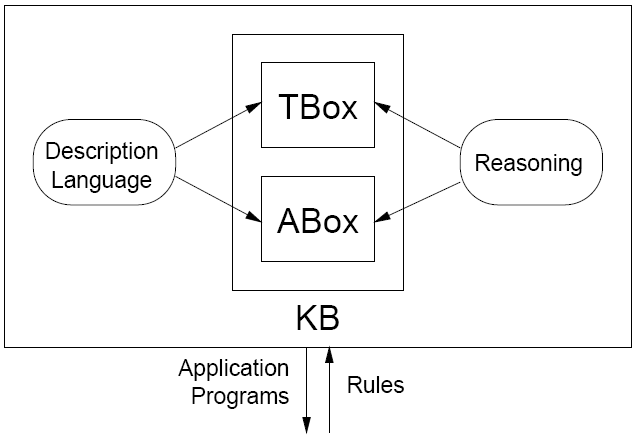
\includegraphics[scale=0.6]{images/chapter2/DLSystemArchitecture}
\caption{The architecture of Knowledge Representation System based on Description Logics \cite{BCM03}}
\label{fig:DLSystemArchitecture}
\end{figure}

\noindent TBox introduces the terminology which means the vocabulary of application domain. The vocabulary consist of \textit{concepts} (set of individuals) and \textit{roles} (binary relationships between individuals). TBox can also be used for creating names (abbreviations) for complex descriptions. ABox contains assertions about named individuals in terms of this vocabulary. When it comes to searching analogies for understanding what TBox and ABox component is, we can collate TBox part with database \textit{schema}, and ABox with database \textit{data}.

DL systems, besides storing terminologies and assertions, also provide reasoning mechanisms. Hence, TBox (term classifier) reasons about concepts and roles descriptions and their relationships, while ABox reasons about individuals and their relationships, e.g.
\begin{itemize}
    \item TBox:

\[
\begin{array}{lcl} 
	\mathit{GoodCPU}    & \equiv    & \mathit{Thing} \sqcap~ (\exists \mathit{isMadeOf}.\mathit{Metalloid}) \\ 
                        &           & \sqcap~ (\exists \mathit{isCreatedBy}.\mathit{ChipManufacturer}) \\
                        &           & \sqcap~ (\forall \mathit{hasFeature}.(\geq 4~ \mathit{hasCore} \sqcup \lnot \mathit{x86Arch})) \\
                        &           & \sqcap~ \exists \mathit{hasFeature}.\top
\end{array}
\]

In one of its simplest form TBox introduces abbreviation for a complex description. The abbreviation here is $\mathit{GoodCPU}$, which indicates something described by following statement: "a thing made of semi metal, which is created by chip maker and all of its features are either more than 3 cores or not x86 architecture".

\newpage
    \item ABox:

\[
\begin{array}{ll} 
    \mathit{GoodCPU}(\mathit{Itanium})              & \mathit{Metalloid}(\mathit{Silicon}) \\
    \mathit{ChipManufacturer}(\mathit{Intel Corp.}) & \mathit{hasFeature}(\mathit{Itanium}, \mathit{IA64}) \\
    \mathit{hasCore}(\mathit{Itanium}, 12)          & \lnot \mathit{x86Arch}(\mathit{IA64})
\end{array}
\]

We can see descriptions of specific situation, where properties are asserted for some individuals. $\mathit{GoodCPU}$ indicates the "Itanium chip made of Silicon by Intel Corporation, which has 12 cores based on IA64 architecture (not backward compatible with old x86)".

\end{itemize}

\noindent Reasoning about terminology (TBox) provides \textbf{satisfiability} (i.e. non-contradictory) and \textbf{subsumption} services. Satisfiability is used for finding an interpretation that makes the formula true and subsumption is used for organizing the concept hierarchy according to their generality (ordering of concepts based on subsumption relation). 

Reasoning about assertions (ABox) provides \textbf{consistency} and \textbf{instantiation} mechanisms. A theory is consistent when it does not contain contradiction. In the semantic terms it means, that it has a model. Instantiation is used to perform \textit{realization} and \textit{retrieval}. Realization means computing the most specific concepts which an individual instantiates while retrieval means computing the individuals which are instances of a given concept. 

Satisfiability checks of descriptions while consistency checks of sets of assertions to determine whether a knowledge base is meaningful or not.

On the start of typical DLKRS application, TBox reasoning services are invoked to ensure that all defined concepts are satisfiable, i.e. are not subsumed by the bottom concept, which is always interpreted as the empty set. Moreover, subsumption hierarchy is computed. This hierarchy would then be inspected to make sure that it coincides with the intention of the modeler. Next it comes to ABox, which first check for its consistency with the TBox and then, for example, compute the most specific concepts that each individual is an instance of (known as realizing the ABox).

\subsection{Description languages}
\label{sub:DLs}

As it was mentioned at the beginning, elementary descriptions are the expressions built from \textit{atomic concepts} (unary predicates) and \textit{atomic roles} (binary predicates). Complex descriptions are created from elementary descriptions inductively by using of \textit{concept constructors}.

Description languages are distinguished by the constructors they provide. The language $\mathcal{AL}$ (Attributive Language) is a minimal language of practical interest. The other languages of this family are extensions of $\mathcal{AL}$, i.e. $\mathcal{ALC}$ (Section \ref{sss:ALC}) is obtained from $\mathcal{AL}$ by adding the complement operator $(\lnot)$, $\mathcal{ALE}$ is obtained from $\mathcal{AL}$ by adding existential restrictions $(\exists R.C)$, etc. \cite{BCM03, HLP08}. Before moving into details, we will introduce conventional notation in DL:

\newpage

\begin{table}[htp]
\centering
\begin{tabular}{ |c|l| }
    \hline
    \textbf{Symbol} & \multicolumn{1}{c|}{\textbf{Description}} \\ \hline
    $\top$          & all concept names \\ \hline
    $\bot$          & empty  concept \\ \hline
    $\sqcap$        & intersection or conjunction of concepts \\ \hline
    $\sqcup$        & union or disjunction of concepts \\ \hline
    $\lnot$         & negation  or complement of concepts \\ \hline
    $\forall$       & universal restriction \\ \hline
    $\exists$       & existential restriction \\ \hline
    $\sqsubseteq$   & concept inclusion \\ \hline
    $\equiv$        & concept equivalence \\ \hline
    $\doteq$        & concept definition \\ \hline
    $:$             & concept/role assertion \\ \hline
\end{tabular}
\caption{DL notation}
\end{table} 

\noindent Let A and B be atomic concepts, R be atomic role, and C and D be concept descriptions. Based on that abstract notation, concept descriptions in $\mathcal{AL}$ language are formed by following syntax rule \cite{BCM03}:

\smallskip

\[
\begin{array}{lcll} 
    C,D & \to   & A~|               & (atomic~ concept) \\ 
        & 		& \top~|            & (universal~ concept) \\
        & 		& \bot~|            & (bottom~ concept) \\
        &		& \lnot A~|         & (atomic~ negation) \\
        &		& C \sqcap D~|      & (intersection) \\
        &		& \forall R.C~|     & (value~ restriction) \\
        &		& \exists R.\top~|  & (limited~ existential~ quantification)
\end{array}
\]

\smallskip

In this section a basic example of what can be expressed using $\mathcal{AL}$ is shown. Let's assume $\mathbf{Computer}$ and $\mathbf{Notebook}$ are atomic concepts. Based on that $\mathbf{Computer} \sqcup \mathbf{Notebook}$ is an $\mathcal{AL}-concept$ describing computers which are notebooks. In analogical way $\mathbf{Computer} \sqcup \lnot\mathbf{Notebook}$ describes concept of computers which are not notebooks (they can be calculators, supercomputers, etc.). Suppose $\mathbf{hasConnection}$ is an atomic role - we can describe the concept $\mathbf{Computer} \sqcap \exists\mathbf{hasConnection}.\top$ as indicating computers which have network connections. $\mathbf{Computer} \sqcap \forall\mathbf{hasConnection}.\mathbf{Notebook}$ describes such computers which are connected only to other notebooks. Concept of computers without any connections is $\mathbf{Computer} \sqcap \forall\mathbf{hasConnection}.\bot$.

When it comes to define semantics of $\mathcal{AL}-concepts$ we consider interpretation $\mathcal{I}$. The interpretation consists of a non-empty set $\Delta^{\mathcal{I}}$ (the domain of the interpretation) and an interpretation function, which assigns to every atomic concept $A$ a set $A^{\mathcal{I}} \subseteq \Delta^{\mathcal{I}}$ and to every atomic role $R$ a binary relation $R^{\mathcal{I}} \subseteq \Delta^{\mathcal{I}} \times \Delta^{\mathcal{I}}$. The interpretation function is extended to concept descriptions by the following inductive definitions \cite{BCM03}:

\newpage

\[
\begin{array}{rcl}
    \top^{\mathcal{I}}              & = & \Delta^{\mathcal{I}} \\
    \bot^{\mathcal{I}}              & = & \emptyset \\
    (\lnot A)^{\mathcal{I}}         & = & \Delta^{\mathcal{I}}\setminus A^{\mathcal{I}} \\
    (C\sqcap D)^{\mathcal{I}}       & = & C^{\mathcal{I}}\cap D^{\mathcal{I}} \\
    (\forall R.C)^{\mathcal{I}}     & = & \{a \in \Delta^{\mathcal{I}}~|~\forall b.~(a,b) \in R^{\mathcal{I}} \to b \in C^{\mathcal{I}}\} \\
    (\exists R.\top)^{\mathcal{I}}  & = & \{a \in \Delta^{\mathcal{I}}~|~\exists b.~(a,b) \in R^{\mathcal{I}}\}
\end{array}
\]

\smallskip

Two concepts $C$, $D$ are equivalent ($C \equiv D$), if $C^{\mathcal{I}} = D^{\mathcal{I}}$ for all interpretations $\mathcal{I}$, e.g. $\forall hasConnection.Notebook \sqcap \forall hasConnection.Ebook$ is equivalent to $\forall hasConnection.(Notebook \sqcup Ebook)$.

\subsubsection{Syntax and semantics of \texorpdfstring{$\mathcal{ALC}$}{ALC}} %  bookmarks are just strings of characters (no formatting instructions are allowed), so use best approximation possible for them (second arg of \texorpdfstring)
\label{sss:ALC}

The basic DL $\mathcal{ALC}$ stands for \textbf{Attributive Concept Language with Complements}. It was introduced by Manfred Schmidt-Schauß and Gert Smolka in 1991. $\mathcal{ALC}$ is obtained from $\mathcal{AL}$ by adding the complement operator $(\lnot)$. Below, there are definitions of syntax and semantics of $\mathcal{ALC}$ \cite{HLP08}:

\bigskip

\begin{definition}\label{alcSyntax} ($\mathcal{ALC}$ syntax). Let $N_{C}$ be a set of concept names and $N_{R}$ be a set of role names. The set of $\mathcal{ALC}$-concept descriptions is the smallest set such that

\begin{enumerate}
    \item $\top$, $\bot$, and every concept name $A\in N_{C}$ is an $\mathcal{ALC}$-concept description,
    \item if $C$ and $D$ are $\mathcal{ALC}$-concept descriptions and $r\in N^{R}$, then $C \sqcap D$, $C \sqcup D$, $\lnot C$, $\forall r.C$, and $\exists r.C$ are $\mathcal{ALC}$-concept descriptions.
\end{enumerate}

\noindent In the following, we will often use "$\mathcal{ALC}$-concept" instead of "$\mathcal{ALC}$-concept description". The semantics of $\mathcal{ALC}$ (and of DLs in general) is given in terms of interpretations.
\end{definition}

\medskip

\begin{definition}\label{alcSemantics} ($\mathcal{ALC}$ semantics). An interpretation $I = (\Delta^{\mathcal{I}},\cdot^{I})$ consists of a nonempty set $\Delta^{\mathcal{I}}$, called the domain of $\mathcal{I}$, and a function $\cdot^{\mathcal{I}}$ that maps every $\mathcal{ALC}$-concept to a subset of $\Delta^{\mathcal{I}}$, and every role name to a subset of $\Delta^{\mathcal{I}} \times \Delta^{\mathcal{I}}$ such that, for all $\mathcal{ALC}$-concepts $C$,$D$ and all role names $r$,

\smallskip

\[
\begin{array}{rcl}
    \top^{\mathcal{I}}          & =	& \Delta^{\mathcal{I}} \\
    \bot^{\mathcal{I}}          & =	& \emptyset \\
    (C\sqcap D)^{\mathcal{I}}   & =	& C^{\mathcal{I}}\cap D^{\mathcal{I}} \\
    (C\sqcup D)^{\mathcal{I}}   & =	& C^{\mathcal{I}}\cup D^{\mathcal{I}} \\
    (\lnot C)^{\mathcal{I}}     & =	& \Delta^{\mathcal{I}}\setminus C^{\mathcal{I}} \\
    (\forall r.C)^{\mathcal{I}} & =	& \{x \in \Delta^{\mathcal{I}}~|~ For~ all~ y \in \Delta^{\mathcal{I}}~ if~<x,y> \in r^{\mathcal{I}},~ then~ y \in C^{\mathcal{I}}\} \\
    (\exists r.C)^{\mathcal{I}} & =	& \{x \in \Delta^{\mathcal{I}}~|~There~ is~ some~ y \in \Delta^{\mathcal{I}}~ with~ <x,y> \in r^{\mathcal{I}}~ and~ y \in C^{\mathcal{I}}\}
\end{array}
\]

\smallskip

\noindent We say that $C^{\mathcal{I}}~ (r^{\mathcal{I}})$ is the extension of the concept $C$ (role name $r$) in the interpretation $\mathcal{I}$. If $x\in C^{\mathcal{I}}$, then we say that $x$ is an instance of $C$ in $\mathcal{I}$.
\end{definition}

\section{OWL}
\label{sec:owl}

\subsection{Introduction}
\label{sub:owlIntroduction}

The OWL Web Ontology Language (OWL), is an ontology language for the Semantic Web with formally defined meaning. It was released in February 2004 as a W3C recommendation. OWL lays on top of RDF and RDFS and comes with a larger vocabulary and stronger syntax. All of them have similar foundations, but OWL is a stronger language with greater machine interpretability than RDF. It can be used to define classes and properties like RDFS, but contains additional set of constructs, which gives to it more expressive power. OWL 2 ontologies provide classes, properties, individuals, and data values and are stored as Semantic Web documents. OWL ontologies can be used along with information written in RDF, and OWL ontologies themselves are primarily exchanged as RDF documents. \textit{"OWL's expressivity is sufficient to cover most of the well-known Description Logic formalisms"} \cite{HLP08, W3COWL}.

\subsection{DLs and OWL}
\label{sub:dlsAndOwl}

OWL is DL-based ontology language. Because the semantics of OWL (Lite and DL) \textit{"can be defined via a translation into an expressive DL"} \cite{HLP08}, implemented DL reasoners can be used for reasoning tasks in applications built on OWL. Analogies in the naming conventions between DL and OWL, are shown in Table \ref{tab:naming}.

\medskip

\begin{table}[htp]
\centering
\begin{tabular}{ |>{\centering\arraybackslash}m{2cm}|>{\centering\arraybackslash}m{2cm}| }
    \hline
    \multicolumn{1}{|c|}{\textbf{OWL}}  &	\multicolumn{1}{c|}{\textbf{DL}} \\ \hline
    class                               &	concept \\ \hline
    object                              &	individual \\ \hline
    property                            &	role \\ \hline
\end{tabular}
\caption{OWL DL naming synonyms}
\label{tab:naming}
\end{table}

\newpage

\noindent An OWL ontology describes the domain in the terms of classes (concepts), objects (individuals) and properties (roles). OWL classes can be created from basic classes or properties, by variety of constructors. The constructors supported by OWL, are shown in Table \ref{tab:owlConstructors}. An ontology consists of groups of axioms. Axioms are used for making the assertions, e.g. assertions of subsumption relationships between classes or properties. They are presented in Table \ref{tab:owlAxioms}.

\bigskip

\begin{table}[htp]
\centering
\begin{tabular}{ |>{\tt}l|l|l| }
    \hline
    \multicolumn{1}{|c|}{\textbf{Constructor}}  & \multicolumn{1}{c|}{\textbf{DL Syntax}}   & \multicolumn{1}{c|}{\textbf{Example}} \\ \hline
    intersectionOf                              & $C_{1}\sqcap\cdots\sqcap C_{n}$           & $Human \sqcap Male$ \\ \hline
    unionOf                                     & $C_{1}\sqcup\cdots\sqcup C_{n}$           & $\mathit{Doctor} \sqcup \mathit{Lawyer}$ \\ \hline
    complementOf                                & $\lnot C$                                 & $\lnot \mathit{Male}$ \\ \hline
    oneOf                                       & ${x_{1}\cdots x_{2}}$                     & ${\mathit{john},\mathit{mary}}$ \\ \hline
    allValuesFrom                               & $\forall P.C$                             & $\forall \mathit{hasChild}.\mathit{Doctor}$ \\ \hline
    someValuesFrom                              & $\exists r.C$                             & $\exists \mathit{hasChild}.\mathit{Lawyer}$ \\ \hline
    hasValue                                    & $\exists r.\{x\}$                         & $\exists \mathit{citizensOf}.\{\mathit{USA}\}$ \\ \hline
    minCardinality                              & $(\geq nr)$                               & $(\geq 2~\mathit{hasChild})$ \\ \hline
    maxCardinality                              & $(\leq nr)$                               & $(\leq 2~\mathit{hasChild})$ \\ \hline
    inverseOf                                   & $r^{-}$                                   & $\mathit{hasChild}^{-}$ \\ \hline
\end{tabular}
\caption{OWL constructors \cite{HLP08}}
\label{tab:owlConstructors}
\end{table}

\begin{table}[htp]
\centering
\begin{tabular}{ |>{\tt}l|l|l| }
    \hline
    \multicolumn{1}{|c|}{\textbf{Axiom}}    & \multicolumn{1}{c|}{\textbf{DL Syntax}}   & \multicolumn{1}{c|}{\textbf{Example}} \\ \hline
    subClassOf                              & $C_{1} \sqsubseteq C_{2}$                 & $\mathit{Human} \sqsubseteq \mathit{Animal} \sqcap \mathit{Biped}$ \\ \hline
    equivalentClass                         & $C_{1} \equiv C_{2}$                      & $\mathit{Man} \equiv \mathit{Human} \sqcap \mathit{Male}$ \\ \hline
    subPropertyOf                           & $P_{1} \sqsubseteq P_{2}$                 & $\mathit{hasDaughter} \sqsubseteq \mathit{hasChild}$ \\ \hline
    equivalentProperty                      & $P_{1} \equiv P_{2}$                      & $\mathit{cost} \equiv \mathit{price}$ \\ \hline
    disjointWith                            & $C_{1} \sqsubseteq \lnot C_{2}$           & $\mathit{Male} \sqsubseteq \lnot \mathit{Female}$ \\ \hline
    sameAs                                  & ${x_{1}} \equiv {x_{2}}$                  & $\mathit{President\_Bush} \equiv \mathit{G\_W\_Bush}$ \\ \hline
    differentFrom                           & ${x_{1}} \sqsubseteq \lnot {x_{2}}$       & $\mathit{john} \sqsubseteq \lnot \mathit{peter}$ \\ \hline
    TransitiveProperty                      & $P~transitive~role$                       & $\mathit{hasAncestor}~is~a~transitive~role$ \\ \hline
    FunctionalProperty                      & $T \sqsubseteq (\leq 1~P)$                & $T \sqsubseteq (\leq 1~\mathit{hasMother})$ \\ \hline
    InverseFunctionalProperty               & $T \sqsubseteq (\leq 1~P^{-})$            & $T \sqsubseteq (\leq 1~\mathit{isMotherOf}^{-})$ \\ \hline
    SymmetricProperty                       & $P \equiv P^{-}$                          & $\mathit{isSiblingOf} \equiv \mathit{isSiblingOf}^{-}$ \\ \hline
\end{tabular}
\caption{OWL axioms \cite{HLP08}}
\label{tab:owlAxioms}
\end{table}

\newpage

\noindent Based on the DL syntax shown in tables above, we can construct OWL equivalents by serializing them to XML, e.g.

\[
\mathit{Human} \sqcap \mathit{Male}
\]

{\tt \small
\begin{verbatim}
<owl:intersectionOf rdf:parseType="Collection">
   <rdf:Description rdf:about="#Human"/>
   <rdf:Description rdf:about="#Male"/>
</owl:intersectionOf>
\end{verbatim}
}

\[
\mathit{Doctor} \sqcup \mathit{Lawyer}
\]

{\tt \small
\begin{verbatim}
<owl:unionOf rdf:parseType="Collection">
   <rdf:Description rdf:about="#Doctor"/>
   <rdf:Description rdf:about="#Lawyer"/>
</owl:unionOf>
\end{verbatim}
}

\[
\exists \mathit{hasChild}.\mathit{Lawyer}
\]

{\tt \small
\begin{verbatim}
<owl:Restriction>
   <owl:onProperty rdf:resource="#hasChild"/>
   <owl:someValuesFrom rdf:resource="#Lawyer"/>
</owl:Restriction>
\end{verbatim}
}

\[
\exists \mathit{citizensOf}.\{\mathit{USA}\}
\]

{\tt \small
\begin{verbatim}
<owl:Restriction>
   <owl:onProperty rdf:resource="#isCitizenOf"/>
   <owl:hasValue rdf:resource="#USA"/>
</owl:Restriction>
\end{verbatim}
}

\bigskip

\noindent and last, slightly more complicated example:

\[
\begin{array}{lcl} 
    \mathit{GoodCPU}    & \equiv    & \mathit{Thing} \sqcap~ (\exists \mathit{isMadeOf}.\mathit{Metalloid}) \\ 
                        &           & \sqcap~ (\exists \mathit{isCreatedBy}.\mathit{ChipManufacturer}) \\
                        &           & \sqcap~ (\forall \mathit{hasFeature}.(\geq 4~ \mathit{hasCore} \sqcup \lnot \mathit{x86Arch}))
\end{array}
\]

\newpage

{\tt \footnotesize
\begin{verbatim}
<owl:Class rdf:about="#GoodCPU">
   <owl:equivalentClass>
      <owl:Class>
         <owl:intersectionOf rdf:parseType="Collection">
            <rdf:Description rdf:about="&owl;Thing"/>
            <owl:Restriction>
               <owl:onProperty rdf:resource="#createdBy"/>
               <owl:someValuesFrom rdf:resource="#ChipManufacturer"/>
            </owl:Restriction>
            <owl:Restriction>
               <owl:onProperty rdf:resource="#madeOf"/>
               <owl:someValuesFrom rdf:resource="#Metalloid"/>
            </owl:Restriction>
            <owl:Restriction>
               <owl:onProperty rdf:resource="#hasFeature"/>
               <owl:allValuesFrom>
                  <owl:Class>
                     <owl:unionOf rdf:parseType="Collection">
                        <owl:Class>
                           <owl:complementOf rdf:resource="#x86Arch"/>
                        </owl:Class>
                        <owl:Restriction>
                           <owl:onProperty rdf:resource="#hasCore"/>
                           <owl:someValuesFrom>
                              <rdf:Description>
                                 <rdf:type rdf:resource="&rdfs;Datatype"/>
                                 <owl:onDatatype rdf:resource="&xsd;integer"/>
                                 <owl:withRestrictions rdf:parseType="Collection">
                                    <rdf:Description>
                                       <xsd:minInclusive 
                                            rdf:datatype="&xsd;integer">4
                                       </xsd:minInclusive>
                                    </rdf:Description>
                                 </owl:withRestrictions>
                              </rdf:Description>
                           </owl:someValuesFrom>
                        </owl:Restriction>
                     </owl:unionOf>
                  </owl:Class>
               </owl:allValuesFrom>
            </owl:Restriction>
         </owl:intersectionOf>
      </owl:Class>
   </owl:equivalentClass>
</owl:Class>
\end{verbatim}
}

\subsubsection{OWL and reasoners}
\label{sub:owlAndReasoners}

Possibility of using DL reasoning services in OWL-based applications was one of the reasons why OWL is based on DL. \textit{"OWL DL has a formal model-theoretic semantics providing a rigorous and provably decidable semantics for the language"} \cite{HLP08}. The decidability ensures, that consistency of OWL DL ontology can be checked by complete DL reasoners. Reasoners can be also used to infer information from asserted facts. 

Popular reasoners in the OWL community are: FaCT, FaCT++, Pellet, RACER, KAON2 or HermiT (see Section \ref{sss:hermiT}). These systems provide reasoning support for a set of tools designed for ontology creation and maintenance which has already been created. There are: Protégé (used for creation of traffic danger ontology described in Chapter \ref{cha:trafficDangerOntology}), Swoop, OilEd and TopBraid Composer.

Increasing number of tools designed for OWL is both a cause and a motivation for the community, to develop ontologies in many various fields, not only in the scope of the Semantic Web. There are areas like: biology, medicine, geography,
geology, astronomy, agriculture or defense, in which ontologies become adopted \cite{HLP08}.

The specialists from IBM departments in China and USA and Department of Biomedical Informatics in Columbia University, have prepared a report about their experiences with Semantic Web applications \cite{UCEReport}. They were working through large terminology called MED (Medical Entities Dictionary) used at the Columbia Presbyterian Medical Center. MED which previously had been using frame-based logic, has been transformed into OWL ontology. After transformation DL subsumption reasoning service was used to classify that ontology, which has revealed many modeling errors. But, as it is said in the report, \textit{"the important result here is not that we identified these modeling errors due to the increased expressivity of DL. More important is our finding that the missed subsumptions could have cost the hospital many missing results in various decision support and infection control systems that routinely use MED to screen patients."}

\subsection{OWL sublanguages}
\label{sub:owlSublanguages}

W3C specification defines 3 variants of OWL. These sublanguages: OWL Lite, OWL DL, and OWL Full provides different level of expressiveness (increasingly in mentioned order). Each of them contains extensions to its predecessor. Based on scope and complexity of the application domain, appropriate version should be chosen for description of the domain. More complex version gives more freedom in domain modeling. The complexity however affects the cost of a learning, which results in higher learning curve. We have 3 sublanguages inside OWL:
\begin{itemize}
    \setlength{\itemsep}{0cm}
    \setlength{\parskip}{0cm}

    \item \textbf{OWL Lite}, the simplest version, useful enough to support creation of classification hierarchies with simple constraints. It is not widely used and acts as the entry point for Semantic Web application developers.
    \item \textbf{OWL DL}, the most widely used version, includes OWL Lite. It was designed to provide maximum expressiveness possible while retaining computational completeness, decidability, and automated reasoning. That is why OWL DL takes the advantage of reasoning services provided for description logics (see Section \ref{sub:owlAndReasoners}).
    \item \textbf{OWL Full}, the most powerful in expressiveness but also the heaviest in the meaning of a learning cost. Includes OWL DL. Provides different semantic than predecessors.
\end{itemize}

\subsection{OWL 2 versus OWL 1}
\label{sub:owl2vsowl1}

OWL 2 was announced by W3C working group on 27 October 2009, as the extension for previous versions (OWL and OWL 1.1). Like OWL 1, OWL 2 is designed to allow development of ontologies and to simplify this process. The second common design goal is to facilitate sharing ontologies via the web, with the aim of making web content more accessible to machines. Besides, OWL 2 has a very similar overall structure to OWL 1. Figure \ref{fig:owl2Structure} shows main building blocks of OWL 2 and relations between them. Despite changes in naming, almost all the building blocks of OWL 2 were present in OWL 1. All OWL 1 ontologies are valid OWL 2 ontologies.

\medskip

\begin{figure}[htp]
\centering
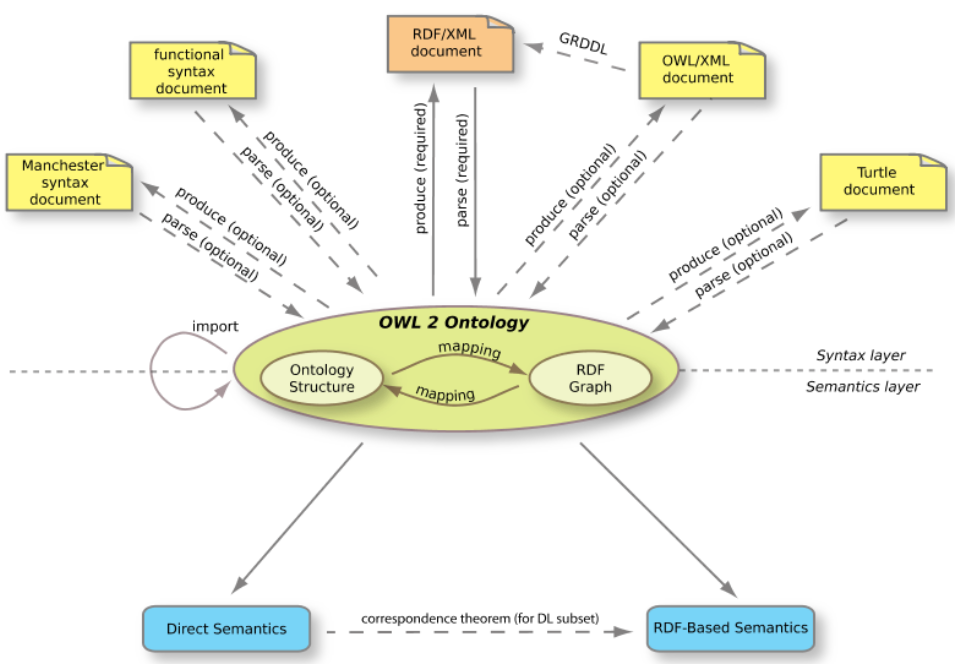
\includegraphics[scale=0.5]{images/chapter2/OWL2Structure}
\caption{The structure of OWL 2 \cite{W3COWL}}
\label{fig:owl2Structure}
\end{figure}

\newpage

\noindent Looking at the structure diagram, we can see that abstract notion of the ontology (abstract structure or RDF graph) is placed in the middle of it. At the top there are various serialization syntaxes for ontologies. At the bottom there are the two semantic specifications. These specifications define the meaning of OWL 2 ontologies. For most of users from the community, only one syntax and one semantic is sufficient. OWL 2 adds some new functionality but still remains compatible with OWL 1. Some of the new features include:
\begin{itemize}
    \setlength{\itemsep}{0cm}
    \setlength{\parskip}{0cm}

    \item keys,
    \item property chains,
    \item richer datatypes, data ranges,
    \item qualified cardinality restrictions,
    \item asymmetric, reflexive, and disjoint properties,
    \item enhanced annotation capabilities.
\end{itemize}

\noindent OWL 2 also defines three new profiles (sublanguages) (OWL 2 EL, OWL 2 QL, OWL 2 RL) and a new syntax (Manchester Syntax). In addition, the set of RDF Graphs that can be handled by DL reasoners is slightly larger in OWL 2 than in its predecessor. It is connected with the fact that some of the restrictions applicable to OWL DL have been relaxed in the newer OWL version \cite{W3COWL}.
